% The dvipsnames option is passed to the xcolor package, which beamer loads
\documentclass[xcolor={dvipsnames}]{beamer}

\usepackage{smpa2152-style}

\title[Qualitative Data]{Qualitative Data}
\author[SMPA 2152]{Data Analysis for Journalism and Political
Communication (Spring 2026)}
\date{Prof. Bell}

\begin{document}

%%%%%%%%%%%%%%%%%%%%%%%%%%%%%%%%%%%%%%%%%%%%%%%%%%%%%%%%%%%%%%%%%%
\frame{
  \titlepage
}

%%%%%%%%%%%%%%%%%%%%%%%%%%%%%%%%%%%%%%%%%%%%%%%%%%%%%%%%%%%%%%%%%%
\frame{\frametitle{Qualitative Data Analysis}
  \begin{itemize}[<+->]
    \item So far, we've focused on quantitative data — things we can count
    \item But what about data that isn't numbers? This is
      \textbf{qualitative data}
    \item There are at least twenty different types of qualitative
      data analysis, including several found in the social sciences:
      \begin{itemize}
        \item Case studies
        \item Ethnography
        \item Content analysis
        \item Mixed-methods
      \end{itemize}
    \item Our goal isn't to find a ``best fit line,'' but to find
      patterns, themes, and meaning from ``thick descriptions'' (Geertz, 1973)
    \item We will focus on one type of qualitative analysis: text analysis
  \end{itemize}
}

%%%%%%%%%%%%%%%%%%%%%%%%%%%%%%%%%%%%%%%%%%%%%%%%%%%%%%%%%%%%%%%%%%
\frame{\frametitle{Text Analysis}
  \only<1-6,8>{
    \begin{itemize}[<+->]
      \item Think of:
        \begin{itemize}
          \item<.-> Interview transcripts
          \item Open-ended survey responses
          \item News articles or social media posts
          \item Focus group notes
        \end{itemize}
      \item The most common way to analyze qualitative data is
        \textbf{thematic coding}
      \item A \textbf{code} is just a descriptive label applied to a
        piece of text
      \item We can then quantify our codes: how frequently each code
        appears, in which parts of the text, from which speakers, etc.
    \end{itemize}
  }
  \only<7>{
    \centering
    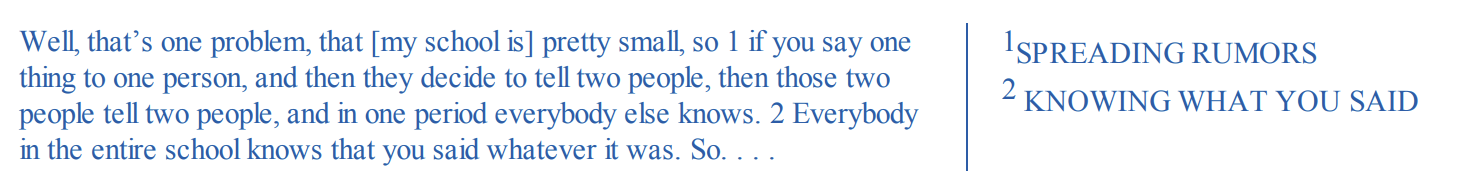
\includegraphics[width = \textwidth]{process_coding_huberman_etal.png}
  }
}

%%%%%%%%%%%%%%%%%%%%%%%%%%%%%%%%%%%%%%%%%%%%%%%%%%%%%%%%%%%%%%%%%%
\frame{\frametitle{Where Do Codes Come From?}
  \begin{itemize}[<+->]
    \item \textbf{Deductive Coding:} You start with a list of codes
      \textit{before} you read
      \begin{itemize}
        \item<.-> This is most often used when the goal of the study
          is to count the appearances of a discrete set of themes,
          e.g., "How often does Donald Trump talk about trade in his speeches?"
      \end{itemize}
    \item \textbf{Inductive Inductive:} You start \textit{without} a
      list fo codes. You read the data and let the themes emerge from the text
      \begin{itemize}
        \item<.-> Many qualitative research studies do not begin with
          well-defined hypotheses, and researchers generate new ideas
          through the process of coding
      \end{itemize}
    \item Most studies begin with a short list of deductive codes,
      then refine those codes or add new ones as you explore the data
  \end{itemize}
}

%%%%%%%%%%%%%%%%%%%%%%%%%%%%%%%%%%%%%%%%%%%%%%%%%%%%%%%%%%%%%%%%%%
\frame{\frametitle{In-Class Exercise}
  \only<1>{
    \textit{\textbf{From StoryCorps}}:\\
    ~\\
    In February of 2012, Jamal Faison was a 20-year-old college
    sophomore home on school break in New York City when he, along
    with two others, were arrested for attempting to steal mobile
    devices from a subway rider. Transit police arrested Jamal and he
    spent the next eight months on Rikers Island — New York City’s
    massive main jail complex.\\
    ~\\
    In September 2012, Jamal pleaded guilty to grand larceny and
    attempted robbery charges and a month later was released from
    custody. Jamal came to StoryCorps to remember the night he was
    released from Rikers, and to discuss his relationship with his uncle, Born.
  }
  \only<2>{
    \inserttimer{5}
  }
}

%%%%%%%%%%%%%%%%%%%%%%%%%%%%%%%%%%%%%%%%%%%%%%%%%%%%%%%%%%%%%%%%%%
\frame{\frametitle{What If We Have Too Much Text?}
  \begin{itemize}[<+->]
    \item Thematic coding by hand is great for 20 interviews, but
      what if we have 20,000 news articles? 2 million tweets?
    \item This is where computational text analysis comes in
    \item When working with computational text analysis, we call the
      full set of text and documents the \textbf{corpus}
    \item The techniques we will learn in this class are called ``bag
      of words'' techniques, because unlike an LLM, they are agnostic
      about the order of the words
      \begin{itemize}
        \item As if you are putting all the words into a bag, drawing
          them out at random, and seeing how frequently they occur
      \end{itemize}
  \end{itemize}
}

%%%%%%%%%%%%%%%%%%%%%%%%%%%%%%%%%%%%%%%%%%%%%%%%%%%%%%%%%%%%%%%%%%
\frame{\frametitle{LDA Topic Modeling}
  \begin{itemize}[<+->]
    \item \textbf{LDA} (Latent Dirichlet Allocation) is a popular method
    \item It is an unsupervised method: you don't give it a list of
      codes. It finds the themes (called ``topics'') made up of words
      that tend to appear together frequently
    \item The researcher must decide what the semantic meaning of
      these topics (correlated words) mean
  \end{itemize}
}

%%%%%%%%%%%%%%%%%%%%%%%%%%%%%%%%%%%%%%%%%%%%%%%%%%%%%%%%%%%%%%%%%%
\frame{\frametitle{Researcher Choices in LDA}
  \begin{enumerate}[<+->]
    \item How many topics?
      \begin{itemize}
        \item You must pre-define how many topics to create
        \item Too few: The topics might be too broad and meaningless
        \item Too many: The topics might be too specific, overlap, or be junk
        \item This is a critical choice with no single right answer
      \end{itemize}
    \item What do the topics mean?
      \begin{itemize}
        \item LDA just gives you a list of words: ``economy,''
          ``jobs,'' ``growth...''
        \item Is that topic ``The Economy''? Or ``Labor Market
          Reports''? Or ``Political Talking Points''?
        \item The researcher must interpret and label the topic. This
          is a subjective, human step!
      \end{itemize}
  \end{enumerate}
}

%%%%%%%%%%%%%%%%%%%%%%%%%%%%%%%%%%%%%%%%%%%%%%%%%%%%%%%%%%%%%%%%%%
\frame{\frametitle{In-Class Exercise}
  \begin{itemize}
    \item Data at:
      \href{https://www.kaggle.com/datasets/christianlillelund/donald-trumps-rallies}{Kaggle.com}
    \item Tool: \href{https://voyant-tools.org/}{Voyant}
  \end{itemize}

}

\end{document}
